% !TEX root = ../report.tex

\chapter{Evaluation}

\minitoc

This chapter will be used to evaluate the work and the results drawn from the research done. This chapter will also discuss why the outcome ended up as it did. This includes obstacles met during research, design and implementation, how issues could have been handled in a different way and significants of the findings.

\clearpage


\section{Development Process}
The development process used in the project was not modelled after any particular rigid paradigm of development, but instead followed the natural workflow of the individual programmers. Even though a particular type of predetermined workflow was not applied, there were clear tendencies in how the development happened.

The team started out with less rigid requirements. In the beginning of the project, they were something along the lines of: Store the netflix movies in an accessible database, retrieve tweets about movies from twitter and store them in the same database.

Each of these requirements were attacked by gathering ruby gems that seemed like they would be suitable for fulfilling the requirement. A proof of concept implementing the requirement was then created in an environment separate from other parts of the project.

As time progressed and more requirements were fulfilled the implementations of the requirements were fused into a larger project. As this project increased in complexity, and the requirements were fulfilled, more requirements emerged. They were implemented and added to the larger code base.

At one point, the code base was beginning to get complex and fusing implementations of requirements into this code base was getting difficult. This implied the need of an architecture. A basic architecture was created and the code was refactored. This process continued looping. An illustration can be seen in figure~\ref{figure:development-cycle}

\begin{figure}[H]
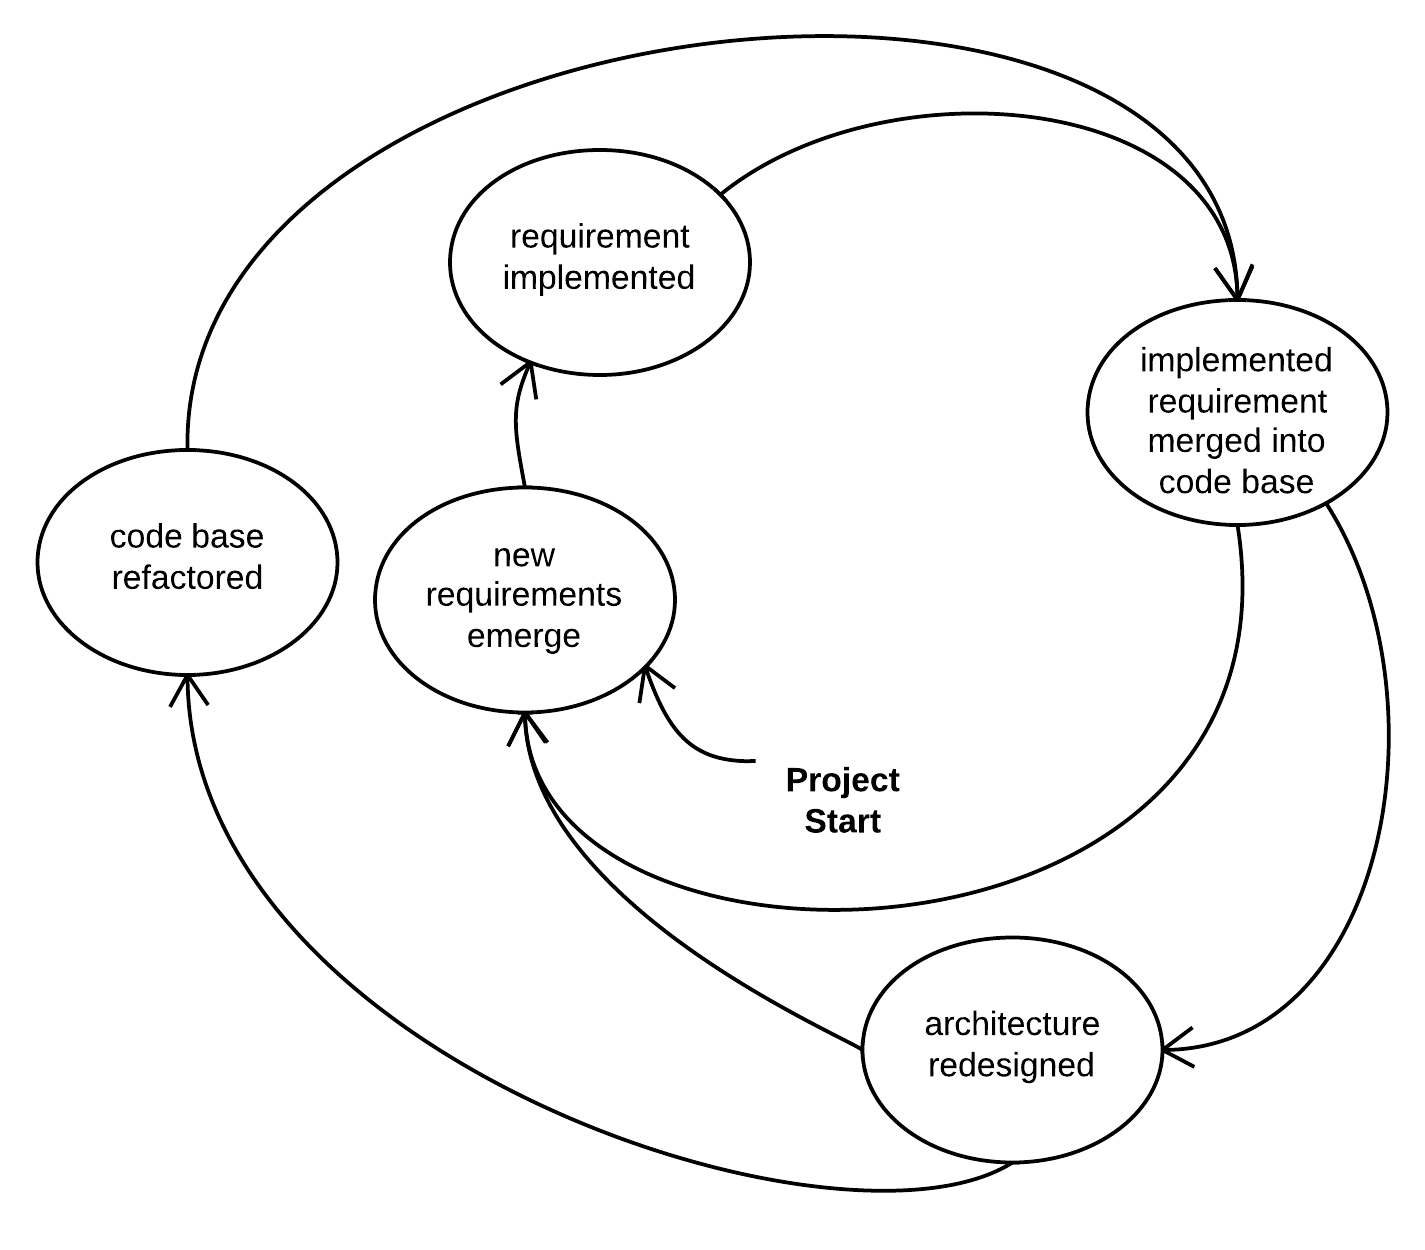
\includegraphics[width=4in]{image/evaluation-development-cycle.png}
\centering
\caption[]{The development cycle that emerged naturally from the individual developers workflow.}
\label{figure:development-cycle}
\end{figure}

\subsection*{Good}
The approach taken was very much a learn as you go-approach. Building an architecture as a first step in the design process can be a good choice. This approach is easier if the architects have extensive knowledge of the systems involved. As this was not the case, the approach allowed the developers to build their knowledge of the existing systems and gems as they went along. Once a knowledge base was reached, a more informed basic architecture could be created.

Doing some implementation early on also reduced the number of pointless goals. If a goal or requirement is created without knowledge of the systems involved, it is likely that the goal will not be reached or that it takes the design in a direction that does not solve other larger goals and requirements.

\subsection*{Bad}
The project went through some major refactoring during development when the architecture was first designed. This was a difficult and time consuming task. An improvement could be made in doing this sooner, but not too soon.

Implementing the requirements outside of the code base made integration more difficult than if the requirement had been implemented within the code base in the first place.

\section{Result Evaluation}
TODO



\section{Issues}
TODO

\subsection*{Group size}
The biggest issue the team encountered was that the team size ended at four. The intended group size for the project was five to seven, which should have produced an extra 325 - 975 work hours, which is a considerable amount of hours. We managed to come out on top of this situation because of a set of responses and effects of having a small group.

\subsubsection*{Ease of communication}
Since we were of such a small size the communication was tight and keeping everyone updated was easy to achieve. This made production efficiency high since there was not done any double work.

\subsubsection*{The team members}
Taking responsibility came more naturally with such a small group as ours. The members stepped up their game and rmivered when it was needed. The general goal of the team was to rmiver a good result. This together with a great chemistry between the members made producing a good result with a small group size achievable.

\subsubsection*{Risk handling}
Since we were dealing with a prototype project, we always had in mind that requirements could change, and therefore had ease of modifiability in the back of our mind, while developing the system.



\section{Summary}
TODO
The course has all in all proved to be a positive and valuable experience for us all. For most of us, the experience of working on such a big project in a team was quite new. We experienced how important it was to plan ahead, to distribute the workload, and to collaborate to achieve a common goal. This was also our first experience in working with an external customer, giving us valuable experiences in this type of project. These experiences are sure to prove useful for in the years to come when we participate in similar projects.

We, as a group, feel that we have reached our goal, and rmivered a great product that the customer was very satisfied with. We made our customer happy and exceeded his expectations, and looking back this achievement is something we can be proud of.
